\section{Pattern Matching DTW}

\newcommand{\dtw}{\mathrm{DTW}}
\newcommand{\ed}{\mathrm{ED}}
\newcommand{\RLE}{\mathrm{RLE}}

\begin{frame}
    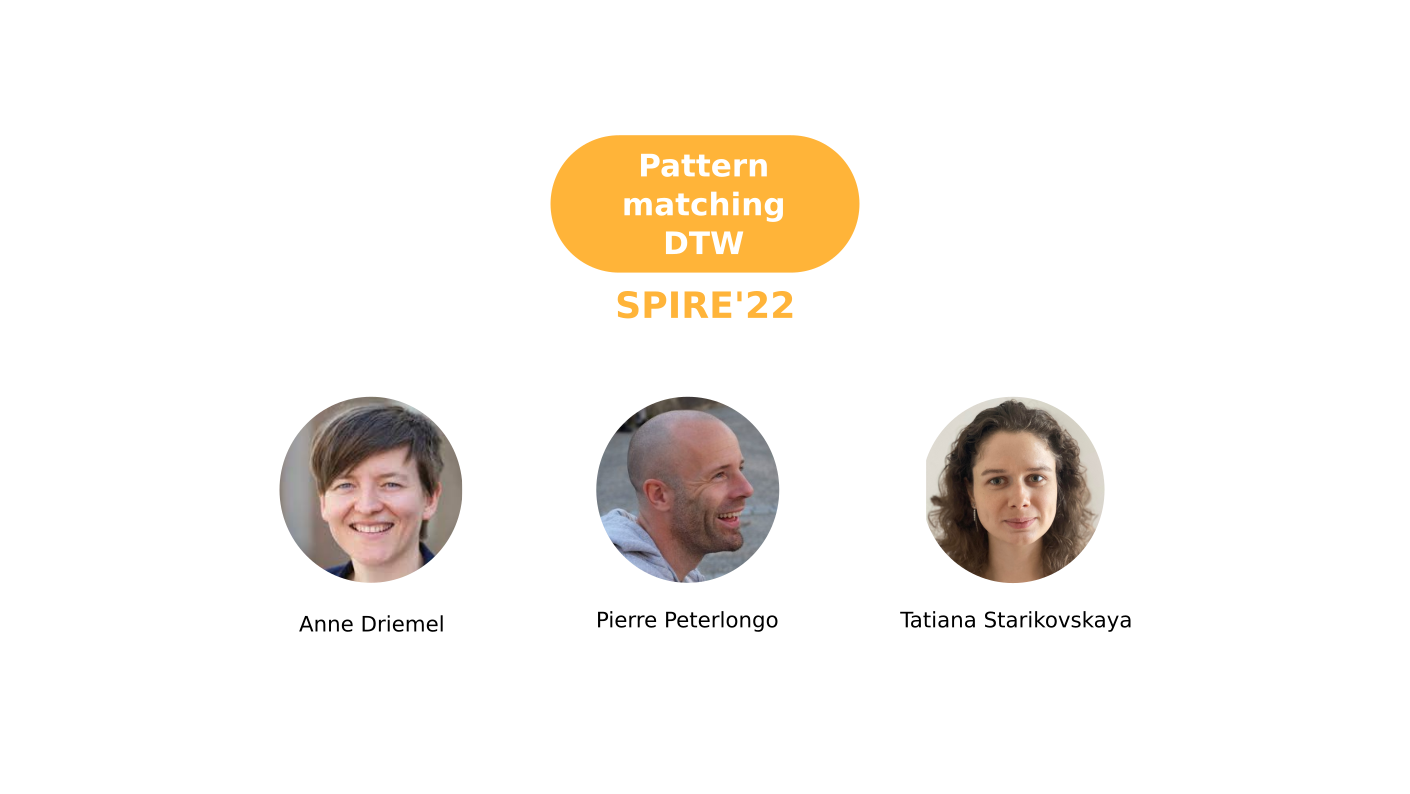
\includegraphics[width=\textwidth]{pictures/mindmap/dtw.png}
\end{frame}


\begin{frame}{Dynamic time warping (DTW) distance }

A \ntheme{measure of similarity between two temporal sequences} which can vary in speed.

\btheme{Definition:} Minimal distance obtained by \ntheme{duplicating} some items of the sequences (maintaining equal length) and then \ntheme{summing the distances} between items at the same position.

\begin{center}
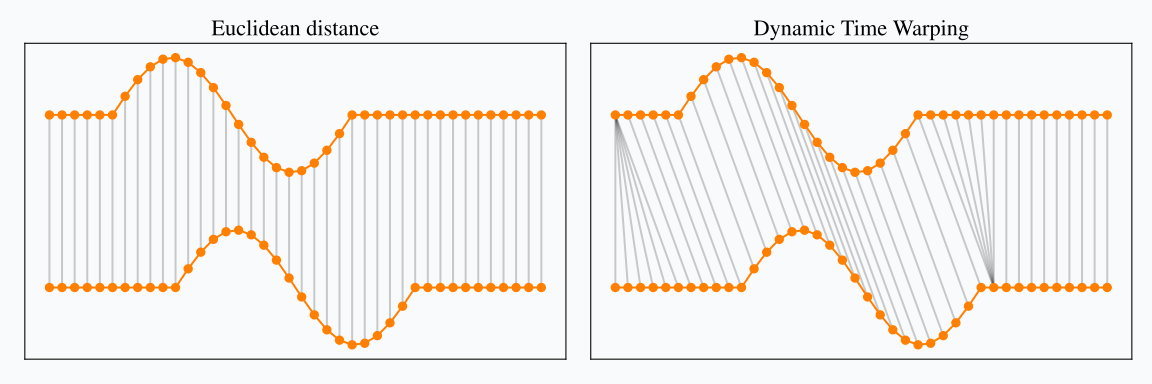
\includegraphics[scale=0.3]{figures/dtw_vs_euc.png}\\
\footnotesize{Figure credit: Romain Tavenard}
\end{center}
\pause
Used in speech recognition to deal with varying speaking speeds.\pause

Studied heavily for \ntheme{parametrized curves} where each item is a multidimensional point.

We focus on \ntheme{strings}, the element of the sequence are characters from $\Sigma$.

\end{frame}

\begin{frame}{Formal definition of $\dtw(X,Y)$ and dynamic programming}

\begin{columns}
\column{0.45\textwidth}
\newcommand{\dtwgrid}[2]{% height width 
\foreach \i in {0,...,#1} {
	\foreach \j in {0,...,#2} {
		\filldraw[black] (\i , \j) circle (2pt);
		\ifthenelse{ \not \equal{#2}{\j}}{ 
			\draw[->] ($(\i , \j+0.9)$) -- ($(\i , \j+0.1)$);
		}{}
		\ifthenelse{ \not \equal{#1}{\i}}{
  			\draw[->] ($(\i +0.1 , \j)$) -- ($(\i +0.9 , \j)$);
		}{}
		\ifthenelse{\not\equal{#1}{\i} \and \not \equal{#2}{\j}}{%
  			\draw[->] ($(\i +0.1 , \j + 0.9)$) -- ($(\i +0.9, \j + 0.1)$);
  		}{}
	}
}
}

\newcommand{\dtwarrow}[2]{%
\draw[->,line width=0.3mm,red] #1 -- #2;
}

\begin{figure}
    \beamermathcolor{black}
    \centering
    \begin{tikzpicture}[scale=0.8, every node/.style={scale=1.2}]
    \dtwgrid{5}{2}

    \foreach \i in {1,...,6} {
        \node at ($(\i-1, 2.8)$) {\tiny{$X[\i]$}};
    }
    \foreach \j in {1,...,3} {
        \node at ($(-1.2, 3 -\j )$) {\tiny{$Y[\j]$}};
    }

    \foreach \x[count=\i] in {C,A,A,A,G,G} {
        \node at ($(\i-1 , 2.3)$) {\textcolor{black}{\tiny{\x}}};
    }
    \foreach \y[count=\j] in {A,T,G} {
        \node at ($(-0.5, 3 -\j )$) {\textcolor{black}{\tiny{\y}}};
    }


    \only<2->{
        \dtwarrow{(0.1,2)}{(0.9,2)}
        \dtwarrow{(3.1,1.9)}{(3.9,1.1)}
        \dtwarrow{(1.1,2)}{(1.9,2)}
        \dtwarrow{(2.1,2)}{(2.9,2)}
        \dtwarrow{(4,0.9)}{(4,0.1)}
        \dtwarrow{(4.1,0)}{(4.9,0)}
        \node at (5,-0.3) {\bred{$\pi$}};
    }

    \end{tikzpicture}
\end{figure}
\column{0.45\textwidth}
\centering
\only<3>{
$\text{cost}(\pi) = \sum_{(i,\ j)\in \pi} d(X[i],Y[j])$\\
\vspace{0.5cm}
$\dtw(X,Y) = \min_{\pi} \text{cost}(\pi)$\\
\vspace{0.5cm}
{\small s.t. $\pi$ goes from top left to bottom right.}}
\end{columns}
\pause %grid definition 
\pause %draw the path
\pause

\bigskip


\only<4|handout:0>{
\begin{exampleblock}{Path correspondance to alignment}
\center
\begin{figure}
%\missingfigure{Under construction...}
\centering
\begin{tikzpicture}[scale=0.7, every node/.style={scale=1}]
\foreach \x[count=\i] in {C,A,A,A,G,G} {
    \node at ($(\i, 1)$) {\small{\x}};
}
\foreach \y[count=\j] in {A,T,G} {
    \node at ($(0.5+\j*1.5, 0)$) {\small{\y}};
}
% align A
\fill[myblue!25] (2, 0.25) -- (2,0.75) -- (4,0.75) -- (2.1,0.25) -- cycle;
% align G
\fill[myblue!25] (5, 0.25) -- (5,0.75) -- (6,0.75) -- (5.1,0.25) -- cycle;
%draw misalignment
\draw[dashed,red] (1.75, 0.25) -- (1,0.75);
\draw[dashed,red] (3.5, 0.25) -- (5,0.75);
\end{tikzpicture}
\end{figure}
\vfill
$\dtw($CAAAG$,$ATG$)=2$
\end{exampleblock}}

\only<5->{

\btheme{Dynamic Programming solution}\\
\smallskip
$D$ a matrix of size $(M+1)(N+1)$ such that $D[i,j]=\dtw(X[1..i],Y[1..j])$\pause
\bigskip

\btheme{Initialization}~~~$D[0,0]= 0$ and for all $(i,j)$, $D[0,j]=D[i,0]=+\infty$.\\
\pause
\bigskip
\btheme{Recurrence} ~~~ 
    $D[i,j] = \min\{$\beamermathcolor{black}
        $\underbrace{\mathcolor{black!30!blue}{D[i-1,j-1]}}_\text{top-left},
        \underbrace{\mathcolor{black!30!blue}{D[i-1,j]}}_\text{top},
        \underbrace{\mathcolor{black!30!blue}{D[i,j-1]}}_\text{left}$
    $\mathcolor{black!30!blue}{\}+ d(X[i], Y[j])}$.
}

\only<6>{
    For $X$ and $Y$ strings, $N=|X|$ and $M=|Y|$, $\Oh(NM)$ space and time.}

\end{frame}


\begin{frame}{Where DTW may perform better: third generation sequencing}
    \begin{center}
    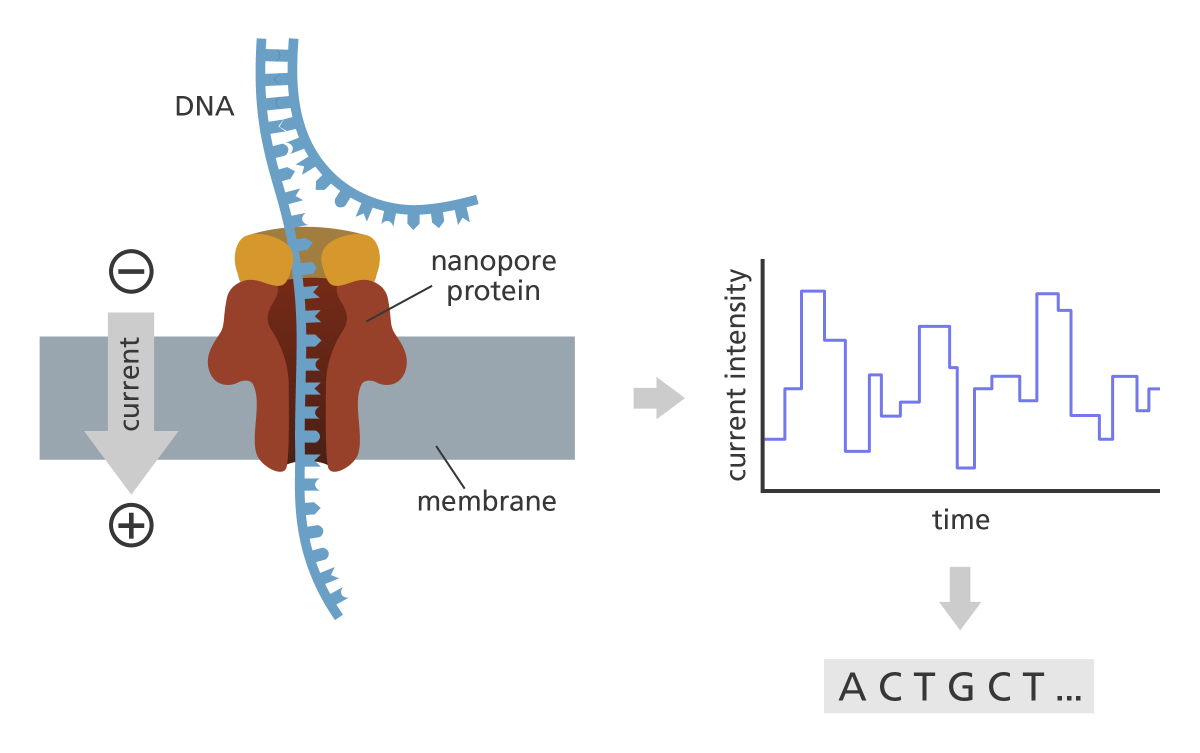
\includegraphics[scale=0.25]{figures/ont-sequencing_yourgenome.png}\\
    \footnotesize{Figure credit: \href{https://www.yourgenome.org/facts/what-is-oxford-nanopore-technology-ont-sequencing/}{yourgenome.org}}
    \end{center}
    
    Uneven speed of the DNA through the nanopore.\pause
    
    Tends to create errors on the homopolymer length...\pause
    
    DTW has been used by [Loose, M., Malla, S. Stout, 2016] and [R. Han, S. Wang, X. Gao, 2020] to try to counter this effect.
    %DTW already used to align the raw signal. We propose using it to aling called reads and provide a visualization of the impact of homopolymer extensions on ED and DTW.
    
\end{frame}

\begin{frame}{Theoretical motivation}
$X$ and $Y$ strings, $N=|X|$ and $M=|Y|$.\\
The dynamic programming takes $\Oh(N^2)$-time if $M=N$. Can we do better?\pause
\begin{block}{No strongly subquadratic [Gold and Sharir]}
%There are no strongly subquadratic algorithms to compute the DTW distance between two strings over a ternary alphabet unless the Strong Exponential Hypothesis (SETH) is false.
$|\Sigma| \geq 3 \Rightarrow $ no $\Oh(N^{a})$ time algorithm with $a<2$ unless SETH is false.
\end{block}\pause

\ntheme{\large Run-length compressed}\\
Let $n$ and $m$ be the number of runs in $X$ and $Y$. \pause
\begin{itemize}
\item General: $\Oh(mN+Mn)$-time [Froese et al.] \pause
\item Binary: $\Oh(nm)$-time [Dupont and Marteau] \pause
\end{itemize} \hfill

\ntheme{\large Low distance regime}\\
Kuszmaul showed how to compute the distance if it is $\leq k$ in $\Oh(kN)$-time.
\end{frame}

\begin{frame}{The effect of runs on the dynamic programming matrix}
\begin{myalertblock}{Theorem 1}
Given $\RLE(P)$ and $\RLE(T)$ and an \textcolor{red}{integer} distance $d: \Sigma \times \Sigma \rightarrow \mathbb{Z}^+$,\\ we can compute all $\dtw$ distances below $k$ in $\Oh(k mn)$ time,\\ where $m=|\RLE(P)|$ and $n=|\RLE(T)|$.
\end{myalertblock}\pause

A subtable $D[i_p .. j_p, i_t .. j_t]$ is called a \bred{\emph{block}} if $P[i_p.. j_p]$ is a run in $P$, and $T[i_t .. j_t]$ is a run in $T$.


%
\begin{center}
\footnotesize
\resizebox{0.8\textwidth}{!}{
\begin{tabular}{|cc||cc|cccc|c|cc|c|cccc|cc|c|c|c|c|c|}
\hline
 &   & G & G & T & T & T & T & C & T & T & A & T & T & T & T & G & G & T & G & A & T & A \\
 & 0 & 0 & 0 & 0 & {0} & 0 & 0 & 0 & 0 & 0 & 0 & 0 & 0 & 0 & 0 & 0 & 0 & 0 & 0 & 0 & 0 & 0 \\
\hline
A  & $\infty$  & 1 & 1 & \textcolor{red}{1} & \textcolor{red}{1} & \textcolor{red}{1} & \textcolor{red}{1} & 1 & 1 & 1 &{ 0 } & 1 & 1 & 1 & 1 & 1 & 1 & 1 & 1 &{ 0 } & 1 &{ 0 }\\
A  & $\infty$  & 2 & 2 & \textcolor{red}{2} & \textcolor{red}{2} & \textcolor{red}{2} & \textcolor{red}{2} & 2 & 2 & 2 &{ 0 } & 1 & 2 & 2 & 2 & 2 & 2 & 2 & 2 &{ 0 } & 1 &{ 0 }\\
\hline
T  & $\infty$  & 3 & 3 &{ 2 } &{ 2 } &{ 2 } &{ 2 } & {3} &{{ 2 }} &{{ 2 }} & 1 &{ 0 } &{ 0 } &{ 0 } &{ 0 } & 1 & 2 &{ 2 } & 3 & 1 &{ 0 } & 1\\
T  & $\infty$  & 4 & 4 &{ 2 } &{ 2 } &{ 2 } &{ 2 } & 3 & {{ 2 }} &{{ 2 }} & 2 &{ 0 } &{ 0 } &{ 0 } &{ 0 } & 1 & 2 &{ 2 } & 3 & 2 &{ 0 } & 1\\
\hline
A  & $\infty$  & 5 & 5 & 3 & 3 & 3 & 3 & 3 & 3 & {3} &{{ 2 }} & 1 & 1 & 1 & 1 & 1 & 2 & 3 & 3 &{ 2 } & 1 &{ 0 }\\
\hline
T  & $\infty$  & 6 & 6 &{ 3 } &{ 3 } &{ 3 } &{ 3 } & 4 &{ 3 } &{ 3 } &{3} &{{ 1 }} &{{ 1 }} &{{ 1 }} &{{ 1 }} & 2 & 2 &{ 2 } & 3 & 3 &{ 1 } & 1\\
\hline

\end{tabular} }
\end{center}





\[
D[i,j] = {\min\{
\underbrace{D[i-1,j-1]}_\text{top-left},
\underbrace{D[i-1,j]}_\text{top},
\underbrace{D[i,j-1]}_\text{left}
\}+ d(X[i], Y[j])
}
\]

Inside a block $d=d(X[i], Y[j])$ is constant.\\ \pause


\begin{block}{Lemma}
\label{lm:non-decreasing}
The values in a block are non-decreasing left-to-right and top-to-bottom.
\end{block}\pause


\end{frame}